% !TeX program = xelatex
% !TeX encoding = UTF-8
\documentclass[journal]{IEEEtran}

\usepackage{amsmath,amssymb,mathtools}
\usepackage{booktabs,array,multirow}
\newcolumntype{C}[1]{>{\centering\arraybackslash}m{#1}}
\usepackage{graphicx}
\usepackage{newtxtext,newtxmath}
\usepackage{enumitem}
\usepackage{placeins}
\usepackage{dblfloatfix}

\usepackage[expansion=false]{microtype}
\usepackage{xurl}
\usepackage{xcolor}
\definecolor{TASECiteBlue}{HTML}{0072B2}
\usepackage[colorlinks=true,citecolor=TASECiteBlue,linkcolor=TASECiteBlue,urlcolor=TASECiteBlue]{hyperref}
\hypersetup{pdfauthor={},pdftitle={Coordinated Scheduling and Process-Mode Selection},pdfsubject={},pdfkeywords={}}
\graphicspath{{figures/}}
\setlength{\emergencystretch}{3em}
\setcounter{topnumber}{2}
\setcounter{dbltopnumber}{2}
\setcounter{dblbotnumber}{1}
\renewcommand{\topfraction}{0.90}
\renewcommand{\dbltopfraction}{0.90}
\renewcommand{\textfraction}{0.10}
\renewcommand{\floatpagefraction}{0.90}
\renewcommand{\dblfloatpagefraction}{0.95}


\usepackage{cite}

\newcommand{\method}{RDMCT-HBS}
\newcommand{\cmax}{C_{\max}}
\newcommand{\pdi}{\mathrm{PDI}}
\newcounter{algorithm}
\newcommand{\algorithmtitle}[1]{\refstepcounter{algorithm}\noindent\textbf{Algorithm~\thealgorithm: #1}\par\smallskip}

\begin{document}
\raggedbottom
\interdisplaylinepenalty=2500
\title{Supplementary Model and Solver Details}
\author{}\maketitle
This supplement accompanies \textit{Coordinated Scheduling and Process-Mode Selection for Dual-Source Rotating-Chamber Cluster Tools}. It expands notation, physical constraints, initial-schedule construction and the learned cut selector. It contains no additional experimental outcomes.
\section{Problem description and two-stage scheduling model}


\subsection{Equipment configuration and scheduling task}

Given the product lot, process modes, wafer-pair layout, and initial equipment state, scheduling determines the start and finish times of loading, alignment, handling, rotation, processing, cleaning, and return actions, together with their order on shared resources. Products depart from LPs and return after processing. Dummies leave vacuum storage, perform filling or cleaning tasks, and return. Robot service, chamber occupancy, and dummy inventory couple the routes.

Inputs comprise action durations, resource capacities, residency limits, cleaning intervals, and dummy counts. Stage one minimizes the final product return time. Stage two improves waiting and cadence under the resulting makespan bound. Each feasible schedule is represented by an action sequence specifying wafers, resources, and start and completion times for performance evaluation and checks of precedence and resource conflicts.

Action durations are deterministic within a solve. No buffers are assumed beyond LPs, aligners, load locks, rotating chambers, and vacuum storage, so each wait corresponds to a material location and resource-occupancy interval.

\subsection{PW-pair modeling for the two process modes}

To represent wafer-level residency and paired handling together, shared transfer and chamber occupancy are modeled at the pair level, while alignment and route timing retain wafer-level events.

A wafer pair (PW pair) is a physical two-wafer transport and chamber-occupancy unit. Its members may be product+product (product PW pair), dummy+dummy (dummy PW pair), or product+dummy (mixed PW pair). Product wafers are preferentially paired by mode and index; an odd tail product may be paired with one dummy, while full-occupancy filling and cleaning may use dummy PW pairs. The sets $\mathcal P^F$ and $\mathcal P^L$ index product-containing PW pairs, including product PW pairs and any required mixed PW pairs. Alignment and residency remain wafer-level operations; the two members share a time window only on a selected two-hand transfer or the same chamber side. The prescribed layout specifies product-containing PW pairing and compatible chamber positions. The MILP optimizes the remaining activation and assignment decisions, physical dummy identities, paired transfers, resource order, and event times within this layout. Legal cleaning segments are generated from the cleaning interval and complete recipe boundaries, after which the MILP activates the cleaning tasks and schedules their times.

A product follows LP--ATR--AL--ATR--upper load lock--VTR--rotary chamber--VTR--lower load lock--ATR--LP: the ATR first places the wafer on the aligner, then retrieves it for transfer into the vacuum domain. A dummy travels from vacuum storage through the VTR to the chamber and returns through the VTR after use. A regular all-product $4\times1$ batch contains two product PW pairs, hence four product wafers, and processes all four positions synchronously once before last-in--first-out unloading; only the last incomplete batch may use a dummy or mixed PW pair to fill all positions. In $2\times2$, every product-containing PW pair occupies two adjacent process cycles so that each of its product members is processed twice. For three product PW pairs, a dummy PW pair D is loaded first, the chamber rotates, and P1 is loaded before D+P1 undergoes chamber processing. Chamber processing then alternates with ``chamber rotation + chain slide'', changing the occupancy successively to P1+P2, P2+P3, and P3+D; P1, P2, and P3 are each processed twice before all wafers are unloaded. Figures~\ref{fig:chain-en} and \ref{fig:parallel-en} show the event sequences.

\begin{figure}[t]
\centering
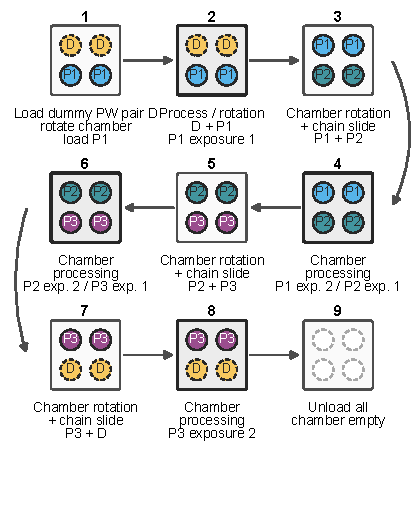
\includegraphics[width=\linewidth]{fig_chain_en_nature}
\caption{$2\times2$ chained processing. A PW pair may be P+P, D+D, or P+D; here each P$i$ is a P+P product PW pair and D is a D+D dummy PW pair. Step 1 loads D, rotates the chamber, and loads P1; Step 2 performs chamber processing on D+P1; Step 3 applies chamber rotation + chain slide to obtain P1+P2. Repeating ``chamber processing--chamber rotation + chain slide'' makes P1, P2, and P3 participate in two adjacent process cycles, so every product wafer is processed twice before all wafers are unloaded.}
\label{fig:chain-en}
\end{figure}

\begin{figure}[t]
\centering
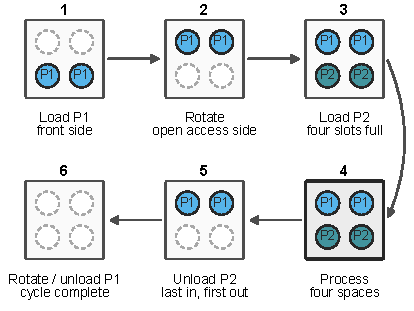
\includegraphics[width=\linewidth]{fig_parallel_en_nature}
\caption{$4\times1$ parallel processing. A regular all-product batch uses two product PW pairs, comprising four product wafers, and receives one synchronous full-occupancy process before last-in--first-out unloading; a dummy or mixed PW pair can complete the final short batch.}
\label{fig:parallel-en}
\end{figure}

Tables~\ref{tab:symbol-en-a} and \ref{tab:symbol-en-b} list the sets, parameters, decision variables, fixed indicators, and derived quantities. The quantities $x^F$, $x^L$, and $\mu^L$ lie in $[0,1]$ and are fixed to zero or one by equality constraints defining the prescribed layout.

\begin{table*}[t]
\centering
\footnotesize
\setlength{\tabcolsep}{2.5pt}
\caption{Core notation I: sets, indices, and input parameters}
\label{tab:symbol-en-a}
\begin{tabular}{C{0.20\textwidth}C{0.20\textwidth}C{0.55\textwidth}}
\toprule
Symbol & Domain and role & Meaning \\
\midrule
$\mathcal S,\mathcal I$ & sets/indices & Material-source interfaces and material units; $i\in\mathcal I$ may be a product or dummy demand.\\
$\mathcal W$ & set/index & Product wafers, indexed by $w$.\\
$\mathcal P^F,\mathcal P^L$ & sets/indices & Product-containing PW pairs assigned to $4\times1$ and $2\times2$; they include P+P product pairs and any required P+D mixed pairs, indexed by $p$.\\
$\mathcal C$ & set/index & Rotary process chambers, indexed by $c$.\\
$\mathcal B_c,\mathcal K_c$ & ordered sets/indices & Candidate $4\times1$ batches $b$ and $2\times2$ product-chain positions $k$ in chamber $c$.\\
$\mathcal L=\{1,2\}$ & set/index & Front and back sides of a $4\times1$ batch.\\
$\mathcal Q_c,\mathcal E_c$ & ordered sets/indices & $2\times2$ process cycles $q$ and cleaning segments $e$ in chamber $c$.\\
$\mathcal V_c$ & set/index & Union of all $4\times1$ batches and $2\times2$ cycles in chamber $c$.\\
$\mathcal O,\mathcal A$ & sets/indices & Candidate physical operations and required process-precedence arcs.\\
$\mathcal R,\Lambda_r$ & sets/indices & Shared resources and physical slots of resource $r$.\\
$\mathcal J_c^D,\mathcal T_c$ & sets/indices & Dummy-wafer demands and reusable physical dummies of chamber $c$.\\
$\chi_{is}$ & known binary constant & Whether material unit $i$ belongs to source interface $s$.\\
$\bar x^F_{pcbl},\bar x^L_{pck}$ & known binary constants & Canonical pair-to-$4\times1$-side or pair-to-$2\times2$-position assignment.\\
$q_c^-(k),q_c^+(k)$ & known nonnegative integer maps & First and second process cycles of $2\times2$ chain position $k$, with $q_c^+(k)=q_c^-(k)+1$.\\
$\bar z_{ce},\bar a^F_{cbe},\bar a^L_{cqe}$ & known binary constants & Active cleaning segments and pre-generated membership of batches or cycles.\\
$H,\bar Q_c$ & nonnegative integer constants & Maximum cycles between cleanings and generated $2\times2$ cycles in chamber $c$.\\
$d_o,\delta_{oo'}$ & nonnegative constants & Duration of operation $o$ and minimum lag on arc $(o,o')$.\\
$d^F_\nu,d^L,r_c$ & nonnegative constants & $4\times1$ stage duration, $2\times2$ process time, and chamber half-rotation time.\\
$\rho^r_{oo'}$ & nonnegative constant & Empty travel or reset time from operation $o$ to $o'$ on resource $r$.\\
$M,\overline R_{wr}$ & positive constants & Valid horizon-based big-$M$ and maximum residency of wafer $w$ in restricted region $r$.\\
$\kappa_o,\Gamma_o$ & integer/set constants & Slots required by operation $o$ and the slots it may use.\\
$\lambda_1,\ldots,\lambda_4$ & nonnegative constants & Stage-two weights for total wait, maximum wait, cadence deviation, and soft-limit excess.\\
$\bar\omega_\alpha,\varepsilon_C$ & nonnegative constants & Soft limit for wait $\alpha$ and the stage-two makespan tolerance.\\
$\mathcal F,\mathcal D_{\rm fix}$ & sets & Full MILP feasible region and discrete indices fixed in stage two.\\
$\mathcal Q^w,\mathcal I_h$ & sets/indices & Wait quantities and process starts admitting cadence second differences.\\
\bottomrule
\end{tabular}
\end{table*}

\begin{table*}[t]
\centering
\footnotesize
\setlength{\tabcolsep}{1pt}
\caption{Core notation II: decision variables, fixed indicators, and derived quantities}
\label{tab:symbol-en-b}
\begin{tabular}{C{0.18\textwidth}C{0.15\textwidth}C{0.47\textwidth}}
\toprule
Symbol & Domain and role & Meaning \\
\midrule
$x^F_{pcbl},x^L_{pck}$ & fixed $[0,1]$ indicators & Product-containing PW-pair placement on a $4\times1$ batch side or at a $2\times2$ chain position.\\
$\mu^L_{pcq}$ & fixed continuous $[0,1]$ alias & Whether $2\times2$ product-containing PW pair $p$ is processed in cycle $q$ of chamber $c$.\\
$u^F_{cb},f^F_{cbl},t^F_{cb}$ & binary variables & $4\times1$ batch activation, dummy filling on a side, and final active batch.\\
$u^L_{ck},a^L_c,v^L_{cq},h^L_{ck}$ & binary variables & $2\times2$ position, chain, process-cycle, and chain-tail activation.\\
$z_{ce},a^F_{cbe},a^L_{cqe},q^{\rm cl}_{ce}$ & fixed indicators/variables & Cleaning segments, task membership, and cleaning-task activation.\\
$\tau_{ce}$ & fixed binary parameter & Whether segment $e$ is the final production segment and exactly exhausts $H$ cycles, thereby triggering terminal cleaning.\\
$q_j,g_{j\tau}$ & binary variables & Dummy demand and assignment to physical dummy $\tau$.\\
$b_o,y^r_{oo'}$ & binary variables & Operation activation and whether $o$ precedes $o'$ on resource $r$.\\
$h_{o\ell}$ & binary slot variable & Whether operation $o$ occupies physical slot $\ell$.\\
$\gamma_{pa}$ & binary variable & Whether pair $p$ uses one paired transfer on robot route $a$.\\
$s_o,e_o$ & nonnegative variables & Start and end times of operation $o$.\\
$s^{F,\nu},e^{F,\nu},s^L,e^L$ & continuous time quantities & Stage-specific notation for $s_o,e_o$ in the two modes.\\
$A^F_{cb},N_{ce}$ & derived continuous/integer quantities & Product-pair count in a $4\times1$ batch and active cycles in a cleaning segment.\\
$a_{vce}$ & fixed binary alias & Whether task $v\in\mathcal V_c$ belongs to cleaning segment $e$.\\
$C_w,C_{\max}$ & nonnegative variables & Product completion time and lot makespan.\\
$\omega_\alpha,L_{\rm sum},L_{\max}$ & nonnegative variables/derived quantities & Stage-two wait or idle quantities, their sum, and their maximum.\\
$\Delta_{ceq},v_{ceq},\eta_\alpha$ & derived/nonnegative variables & Cadence second difference, its absolute-value bound, and soft wait excess.\\
$h_{ceq},\Phi$ & continuous alias/derived objective & Start of the $q$th process in a segment and stage-two schedule-quality objective.\\
$\xi,\widehat\xi,\widehat C$ & vector/stage constants & Current variables, stage-one incumbent, and incumbent makespan.\\
\bottomrule
\end{tabular}
\end{table*}

\subsection{Source interfaces, operation activation, and time relations}

The fixed incidence parameter satisfies
\begin{equation}
\sum_{s\in\mathcal S}\chi_{is}=1,
\qquad i\in\mathcal I.
\label{eq:source-membership-en}
\end{equation}
Equation~\eqref{eq:source-membership-en} assigns each material unit to exactly one source. Setting $|\mathcal S|=1$ gives the single-source tool; using two interfaces and assigning products and dummies to different interfaces gives the dual-source tool.

If $\mathcal A^{\rm int}$ is the internal network and $\mathcal A_s$ contains release and return arcs for source $s$, then
\begin{equation}
\mathcal A=\mathcal A^{\rm int}\cup
\left(\bigcup_{s\in\mathcal S}\mathcal A_s\right).
\label{eq:route-union-en}
\end{equation}
Equation~\eqref{eq:route-union-en} means that one- and two-source tools differ only at route endpoints; processing, cleaning, shared resources, and timing use the same internal model, so a dual-source tool is not the sum of two independent single-source schedules.

Canonical pair positions satisfy
\begin{equation}
\begin{aligned}
x^F_{pcbl}&=\bar x^F_{pcbl}, &
\sum_{c,b,l}x^F_{pcbl}&=1 &&(p\in\mathcal P^F),\\
x^L_{pck}&=\bar x^L_{pck}, &
\sum_{c,k}x^L_{pck}&=1 &&(p\in\mathcal P^L).
\end{aligned}
\label{eq:pair-slot-en}
\end{equation}
Equation~\eqref{eq:pair-slot-en} assigns each wafer pair to one compatible position and fixes equivalent locations to canonical indices. Event times and resource order remain optimization decisions within the prescribed layout.

A position containing a pair must be active, and candidate positions are used consecutively:
\begin{equation}
\begin{aligned}
x^F_{pcbl}&\le u^F_{cb}, &u^F_{c,b+1}&\le u^F_{cb},\\
x^L_{pck}&\le u^L_{ck}, &u^L_{c,k+1}&\le u^L_{ck}.
\end{aligned}
\label{eq:activation-prefix-en}
\end{equation}
Equation~\eqref{eq:activation-prefix-en} activates any batch or chain position containing a product and excludes a nonphysical inactive position followed by an active one.

For each candidate operation $o$, activation and duration satisfy
\begin{equation}
0\le s_o\le Mb_o,\qquad
0\le e_o\le Mb_o,\qquad
e_o=s_o+d_ob_o.
\label{eq:operation-time-en}
\end{equation}
Equation~\eqref{eq:operation-time-en} sets inactive operation times to zero and gives an active operation duration $d_o$. It applies to robot moves, alignment, pump/vent, rotation, product processing, dummy transport, and cleaning.

For every required process arc $(o,o')\in\mathcal A$,
\begin{equation}
b_{o'}\le b_o,\qquad
s_{o'}\ge e_o+\delta_{oo'}-M(2-b_o-b_{o'}).
\label{eq:precedence-en}
\end{equation}
Equation~\eqref{eq:precedence-en} activates a successor only with its predecessor and, when both exist, starts it after the predecessor and minimum lag. These arcs connect product routes, dummy routes, and load--process--unload chains.

\subsection{Occupancy and event order in the two processing modes}

For $4\times1$, let $A^F_{cb}=\sum_{p,l}x^F_{pcbl}$ be the number of product pairs assigned to batch $(c,b)$. Full occupancy and dummy filling are
\begin{equation}
\begin{aligned}
A^F_{cb}&=\sum_{p\in\mathcal P^F}\sum_{l\in\mathcal L}x^F_{pcbl},\\
\sum_{p\in\mathcal P^F}x^F_{pcbl}+f^F_{cbl}&=u^F_{cb}
&& (l\in\mathcal L),\\
\sum_{l\in\mathcal L}f^F_{cbl}&=2u^F_{cb}-A^F_{cb}.
\end{aligned}
\label{eq:full-capacity-en}
\end{equation}
Equation~\eqref{eq:full-capacity-en} gives each active $4\times1$ batch two sides, each occupied by one product pair or one dummy pair; all four chamber positions are therefore filled at process start.

Active batches are consecutive and dummy filling is restricted to the last active batch:
\begin{equation}
\begin{aligned}
A^F_{cb}&\ge u^F_{cb}, &u^F_{c,b+1}&\le u^F_{cb},\\
A^F_{cb}&\ge2u^F_{c,b+1},
&t^F_{cb}&\le u^F_{cb},\\
t^F_{cb}&\le1-u^F_{c,b+1},
&t^F_{cb}&\ge u^F_{cb}-u^F_{c,b+1}.
\end{aligned}
\label{eq:full-tail-en}
\end{equation}
Equation~\eqref{eq:full-tail-en} requires at least one product pair in an active batch and two product pairs if a later batch is active. The last three inequalities set $t^F_{cb}=1$ exactly at the active tail; the final candidate uses $t^F_{cB}=u^F_{cB}$.

Let $FL,BL,P,BU,FU$ denote front load, back load, processing, back unload, and front unload. Then
\begin{equation}
\begin{aligned}
e^{F,\nu}_{cb}&=s^{F,\nu}_{cb}+d^{F}_{\nu}u^F_{cb}
\\[-1pt]&\nu\in\{FL,BL,P,BU,FU\},\\
s^{F,BL}_{cb}&\ge e^{F,FL}_{cb}+r_c-M(1-u^F_{cb}),\\
s^{F,P}_{cb}&=e^{F,BL}_{cb},\\
s^{F,BU}_{cb}&\ge e^{F,P}_{cb}-M(1-u^F_{cb}),\\
s^{F,FU}_{cb}&\ge e^{F,BU}_{cb}+r_c-M(1-u^F_{cb}).
\end{aligned}
\label{eq:full-sequence-en}
\end{equation}
Equation~\eqref{eq:full-sequence-en} loads the front side, rotates to load the back, starts synchronous processing after the back load, and then unloads the back side before rotating and unloading the front. Consecutive batches are linked by $s^{F,FL}_{c,b+1}\ge e^{F,FU}_{cb}-M(1-u^F_{c,b+1})$.

For $2\times2$, each product pair occupies one ordered chain position:
\begin{equation}
u^L_{ck}=\sum_{p\in\mathcal P^L}x^L_{pck},\qquad
u^L_{c,k+1}\le u^L_{ck},\qquad
a^L_c=u^L_{c1}.
\label{eq:mix-position-en}
\end{equation}
Equation~\eqref{eq:mix-position-en} creates a one-to-one relation between product pairs and consecutive chain positions and uses $a^L_c$ to indicate whether chamber $c$ contains a $2\times2$ chain.

Let $q_c^-(k)$ and $q_c^+(k)$ denote the first and second process cycles of chain position $k$. The pair--cycle incidence is
\begin{equation}
\begin{aligned}
q_c^+(k)&=q_c^-(k)+1,\\
\mu^L_{pcq}
&=\sum_{\substack{k\in\mathcal K_c:\\q\in\{q_c^-(k),q_c^+(k)\}}}x^L_{pck},\\
\sum_{q\in\mathcal Q_c}\mu^L_{pcq}
&=2\sum_{k\in\mathcal K_c}x^L_{pck}.
\end{aligned}
\label{eq:mix-two-exposures-en}
\end{equation}
Equation~\eqref{eq:mix-two-exposures-en} maps every assigned $2\times2$ product-containing PW pair to exactly two adjacent process cycles. Every product member inherits the same $\mu^L_{pcq}$ incidence, so a product is not omitted even when an odd tail uses a P+D mixed PW pair. The equation also distinguishes the modes explicitly: a $2\times2$ product-containing pair spans two cycles, whereas two $4\times1$ side pairs are processed once in one full batch.

The generated layout supplies the number $\bar Q_c$ of process cycles, and $h^L_{ck}$ identifies the chain tail:
\begin{equation}
\begin{aligned}
v^L_{cq}&=
\begin{cases}a^L_c,&q\le\bar Q_c,\\0,&q>\bar Q_c,
\end{cases}\\
\sum_k h^L_{ck}&=a^L_c,\qquad
h^L_{ck}\le u^L_{ck},\qquad
h^L_{ck}+u^L_{c,k+1}\le1,\\
h^L_{ck}&\ge u^L_{ck}-u^L_{c,k+1}.
\end{aligned}
\label{eq:mix-layout-en}
\end{equation}
Equation~\eqref{eq:mix-layout-en} gives $n+1$ process cycles for a segment with $n$ product-containing PW pairs: the head is dummy PW pair+P1, internal cycles are P$i$+P$i+1$, and the tail is P$n$+dummy PW pair. The final relations make $h^L_{ck}$ one only at the last active product position.

For a legal chain segment $(q_0,\ldots,q_T)$, let $H_0$, $B_q$, and $T_0$ denote head loading, internal exchange, and tail unloading. Then
\begin{equation}
\begin{aligned}
e^L_{cq}-s^L_{cq}&=d^L v^L_{cq},\\
s^L_{cq_0}&=e^{H_0}_c,\\
s^{B}_{cq}&\ge e^L_{c,q-1}-M(1-a^L_c),\\
s^L_{cq}=e^{B}_{cq}\quad(q_0<q\le q_T),\\
s^{T_0}_c&\ge e^L_{cq_T}-M(1-a^L_c).
\end{aligned}
\label{eq:mix-sequence-en}
\end{equation}
Equation~\eqref{eq:mix-sequence-en} begins the first process immediately after head loading, performs an internal exchange only after the previous cycle, and unloads the tail only after the last process. It directly realizes dummy+P1, P1+P2, $\ldots$, Pn+dummy.

\subsection{Cleaning and reusable dummy wafers}

Cleaning segments are generated from $H$ and complete process boundaries and enter the MILP as fixed binary indicators:
\begin{equation}
z_{ce}=\bar z_{ce},\qquad
a^F_{cbe}=\bar a^F_{cbe}u^F_{cb},\qquad
a^L_{cqe}=\bar a^L_{cqe}v^L_{cq}.
\label{eq:clean-layout-en}
\end{equation}
Equation~\eqref{eq:clean-layout-en} prevents arbitrary cleaning locations: $4\times1$ may split only at batch boundaries and $2\times2$ only after a complete chain segment, while the MILP still schedules process and cleaning times.

Let $N_{ce}$ be the number of active process cycles in segment $e$:
\begin{equation}
\begin{gathered}
N_{ce}=\sum_b a^F_{cbe}+\sum_q a^L_{cqe},\qquad
z_{ce}\le N_{ce}\le Hz_{ce},\\
q^{\rm cl}_{ce}=z_{c,e+1}+\tau_{ce},\qquad z_{c,E_c+1}=0.
\end{gathered}
\label{eq:clean-count-en}
\end{equation}
Equation~\eqref{eq:clean-count-en} places at least one and at most $H$ process cycles in an active segment. It activates an internal cleaning before every subsequent production segment and, when the final segment exactly exhausts $H$ cycles, sets $\tau_{ce}=1$ to activate terminal cleaning. Both are complete equipment actions; only the terminal action has no subsequent product processing.

Let $\mathcal V_c$ be the union of $4\times1$ batches and $2\times2$ cycles and let $a_{vce}$ take the corresponding $a^F$ or $a^L$. Cleaning order and the physical cleaning chain satisfy
\begin{equation}
\begin{aligned}
s_v&\ge e^{\rm cl}_{c,e-1}-M(1-a_{vce}) &&(e>1),\\
e_v&\le s^{\rm cl}_{ce}+M(1-a_{vce})+M(1-q^{\rm cl}_{ce}),\\
s^{\rm cl,BL}_{ce}&\ge e^{\rm cl,FL}_{ce}+r_c-M(1-q^{\rm cl}_{ce}),\\
s^{\rm cl,P}_{ce}&\ge e^{\rm cl,BL}_{ce}-M(1-q^{\rm cl}_{ce}),\\
s^{\rm cl,BU}_{ce}&\ge e^{\rm cl,P}_{ce}-M(1-q^{\rm cl}_{ce}),\\
s^{\rm cl,FU}_{ce}&\ge e^{\rm cl,BU}_{ce}+r_c-M(1-q^{\rm cl}_{ce}).
\end{aligned}
\label{eq:clean-time-en}
\end{equation}
Equation~\eqref{eq:clean-time-en} starts a segment after the preceding cleaning and finishes it before the next cleaning. A cleaning task loads both chamber sides with dummies, rotates, processes, and unloads in reverse, thereby occupying the VTR, chamber, and four physical dummies rather than adding virtual downtime.

Dummy demand $j$ is activated by a physical event:
\begin{equation}
q_j=
\begin{cases}
f^F_{cbl},&j\text{ is a final-$4\times1$ filling demand},\\
a^L_c,&j\text{ is a chain endpoint demand},\\
q^{\rm cl}_{ch},&j\text{ is a cleaning demand}.
\end{cases}
\label{eq:dummy-demand-en}
\end{equation}
Equation~\eqref{eq:dummy-demand-en} prevents dummies from becoming an unlimited abstract filler: a physical demand exists only for a final batch, chain head/tail, or active cleaning task.

Each active demand selects one physical dummy from inventory:
\begin{equation}
\sum_{\tau\in\mathcal T_c}g_{j\tau}=q_j,
\qquad j\in\mathcal J_c^D.
\label{eq:dummy-assign-en}
\end{equation}
Equation~\eqref{eq:dummy-assign-en} assigns every active demand exactly once. Mutual exclusion subsequently orders repeated uses of the same physical dummy, so it can be reused only after unloading and return to storage.

\subsection{Robots, load locks, chambers, and time resources}

ATR, AL, VTR, and each rotary chamber are unary resources; the upper and lower load locks each have two physical slots; each dummy in inventory is a reusable slot. An operation $o$ requiring $\kappa_o$ slots satisfies
\begin{equation}
\sum_{\ell\in\Gamma_o}h_{o\ell}=\kappa_ob_o.
\label{eq:slot-select-en}
\end{equation}
Equation~\eqref{eq:slot-select-en} assigns an active operation the required number of legal physical slots and assigns none to an inactive operation. AL, ATR, VTR, and a chamber have one slot, while load locks and dummy inventory retain physical identities.

If operations $o$ and $o'$ may compete for slot $\ell$ of resource $r$, then
\begin{equation}
\begin{aligned}
s_{o'}&\ge e_o+\rho^r_{oo'}-M(1-y^r_{oo'})
-M(1-h_{o\ell})-M(1-h_{o'\ell}),\\
s_o&\ge e_{o'}+\rho^r_{o'o}-My^r_{oo'}
-M(1-h_{o\ell})-M(1-h_{o'\ell}).
\end{aligned}
\label{eq:resource-order-en}
\end{equation}
Equation~\eqref{eq:resource-order-en} makes $y^r_{oo'}$ choose one order whenever two actions use the same slot and includes empty robot travel or equipment reset through $\rho^r_{oo'}$. It applies to ATR, AL, both load locks, VTR, rotary chambers, and individual dummies, preventing concurrent robot actions and reuse before release.

An individual product or dummy stage must coincide with its selected batch, chain position, or cleaning window. For selection $x$ and reference stage $[s^{\rm ref},e^{\rm ref}]$,
\begin{equation}
\begin{aligned}
-M(1-x)&\le s_o-s^{\rm ref}\le M(1-x),\\
-M(1-x)&\le e_o-e^{\rm ref}\le M(1-x).
\end{aligned}
\label{eq:stage-link-en}
\end{equation}
Equation~\eqref{eq:stage-link-en} synchronizes the individual action with its physical stage when $x=1$ and releases the candidate relation when $x=0$, connecting pair positions, product routes, dummy demands, and chamber windows.

If pair $p$ uses one paired transfer on robot route $a$, the two wafer stages are synchronized:
\begin{equation}
\begin{aligned}
-M(1-\gamma_{pa})&\le s_{w_1a}-s_{w_2a}\le M(1-\gamma_{pa}),\\
-M(1-\gamma_{pa})&\le e_{w_1a}-e_{w_2a}\le M(1-\gamma_{pa}).
\end{aligned}
\label{eq:double-transfer-en}
\end{equation}
Equation~\eqref{eq:double-transfer-en} means that $\gamma_{pa}=1$ moves a complete pair in one non-preemptive robot action. If $\gamma_{pa}=0$, the wafers still occupy the same robot separately and are ordered by Eq.~\eqref{eq:resource-order-en}.

For the entry and exit events of wafer $w$ in restricted equipment region $r$,
\begin{equation}
0\le s_{\operatorname{out}(w,r)}-e_{\operatorname{in}(w,r)}
\le\overline R_{wr}.
\label{eq:residence-en}
\end{equation}
Equation~\eqref{eq:residence-en} limits the physical stay in an upper load lock, chamber, lower load lock, or restricted transport region. Load-lock occupation also spans placement, pump/vent, opposite-side pickup, and pressure reset, so placement by a robot is not mistaken for slot release.

\subsection{Makespan-first two-stage optimization}

Let $C_w$ be the time at which product wafer $w$ completes the lower-load-lock return and reaches its load port. Stage one solves
\begin{equation}
C_w=e_{w,\mathrm{return}},\qquad
C_{\max}\ge C_w\ (w\in\mathcal W),\qquad
\min_{\xi\in\mathcal F}C_{\max}.
\label{eq:primary-objective-en}
\end{equation}
Equation~\eqref{eq:primary-objective-en} measures makespan at the last product wafer's return to LP after its complete end-to-end route. Internal cleaning affects $C_{\max}$ through resource occupancy and precedence that delay subsequent product returns. Terminal cleaning remains in the action sequence, but its completion time does not directly lower-bound $C_{\max}$. It can still affect other chambers' product returns through competition for the shared VTR; this indirect effect is determined by the complete schedule. WPH uses product-return makespan as its denominator. The feasible region $\mathcal F$ is defined by Eqs.~\eqref{eq:source-membership-en}--\eqref{eq:residence-en} expanded over all applicable indices.

Given stage-one incumbent $\widehat\xi$ and makespan $\widehat C$, stage two fixes the discrete structure indexed by $\mathcal D_{\rm fix}$ and minimizes linear schedule quality within the makespan tolerance:
\begin{equation}
\begin{gathered}
\xi_d=\widehat\xi_d\quad(d\in\mathcal D_{\rm fix}),\qquad
C_{\max}\le\widehat C+\varepsilon_C,\\
L_{\rm sum}=\sum_{\alpha\in\mathcal Q^w}\omega_\alpha,\qquad
L_{\max}\ge\omega_\alpha,\\
\Delta_{ceq}=(h_{ce,q+1}-h_{ceq})-(h_{ceq}-h_{ce,q-1}),\\
v_{ceq}\ge\Delta_{ceq},\qquad v_{ceq}\ge-\Delta_{ceq},\\
\eta_\alpha\ge\omega_\alpha-\bar\omega_\alpha,\qquad
\eta_\alpha\ge0,\\
\min\Phi=\lambda_1L_{\rm sum}+\lambda_2L_{\max}
+\lambda_3\sum_{(c,e,q)\in\mathcal I_h}v_{ceq}
+\lambda_4\sum_{\alpha\in\mathcal Q^w}\eta_\alpha.
\end{gathered}
\label{eq:secondary-objective-en}
\end{equation}
Equation~\eqref{eq:secondary-objective-en} preserves the stage-one makespan bound and fixes the principal discrete routes and resource orders. Retained paired-transfer choices and continuous times can change to reduce total wait, maximum wait, and variation between consecutive processing intervals within each segment. Optional soft-limit excess can also be penalized. The experiments use $(\lambda_1,\lambda_2,\lambda_3)=(1,10,25)$ and $\varepsilon_C=10^{-6}$. With the soft waiting limit disabled, no excess variables are generated. For a time-limited first stage, the best incumbent value $\widehat C$ supplies the second-stage bound; variables in $\mathcal D_{\rm fix}$ are fixed while designated paired-transfer variables remain adjustable.

\section{Structure-aware MILP solution framework}

\label{sec:method-new}

The scheduling model couples discrete resource assignments with continuous event times. Primal feasibility requires coordination of full occupancy, dual-source logistics, and shared-resource order, whereas dual-bound improvement depends on valid inequalities acting on discrete choices, continuous times, and their coupling. We exploit these structures through a structure-preserving binary skeleton (SPBS) for initial feasible scheduling and \method{} for cut selection. SPBS supplies a feasible starting point, and \method{} determines cut counts and insertion order. SCIP generates valid cuts, checks feasibility, maintains bounds, and certifies optimality \cite{achterberg2009scip,bestuzheva2023scip}.

The solution process comprises initial-schedule construction and validation, candidate-cut generation, count prediction, ordered-subset search, and role-submodular completion, followed by continued branch-and-bound search. All selected cuts are valid inequalities for the original model and retain their coefficients. Cut selection therefore controls the strengthening of the linear relaxation while preserving the original integer feasible set.

\subsection{SPBS initial solution}

SPBS first constructs a discrete skeleton from the recipe and equipment layout, then solves for event times in a restricted MILP. Product wafers are paired in input order. The $4\times1$ pairs are mapped sequentially to chambers, batches, and front/back positions, whereas the $2\times2$ pairs are assigned round-robin to chamber-chain positions. This determines batch-use, tail-batch, used-position, and last-position indicators. Cleaning counts partition each chamber sequence into process segments: $4\times1$ batches are assigned to their cleaning epochs, while a $2\times2$ chain ends its current segment with process-enabling carriers (PECs) when the cleaning threshold is reached and resumes after cleaning with a new PEC-bounded head. The skeleton therefore determines what is processed, in which chamber, and at which legal cleaning boundary; detailed PEC occupancy and all continuous event times remain governed by the MILP.

At the resource level, SPBS derives a conservative order from the same physical route. ATR first schedules $4\times1$ inputs and returns across chambers and stages the first $2\times2$ pair of a chamber immediately after that chamber's final full batch. It then advances chain inputs and returns segment by segment. Deterministic odd/even load-lock slots break slot symmetry, and the VTR order is aligned with ATR batch progression and cleaning actions. Let $\mathcal F_q$ be the binary variables fixed in relaxation level $q$, with skeleton value $\widehat x_j$. The restricted feasibility subproblem imposes
\begin{equation}
\ell_j^{(q)}=u_j^{(q)}=\widehat x_j,\qquad j\in\mathcal F_q
\label{eq:spbs-fix-en}
\end{equation}
Equation~\eqref{eq:spbs-fix-en} fixes only the skeleton choices at the current level. Start, completion, and waiting times, together with resource orders not fixed at that level, remain free.

SPBS progressively relaxes fixed-variable conditions through five levels, with nested fixed sets $\mathcal F_1\supseteq\mathcal F_2\supseteq\cdots\supseteq\mathcal F_5$. For unchanged skeleton values, releasing these conditions expands the restricted feasible set. If a level yields no feasible solution within its allocated budget, the search proceeds to the next level. The first level fixes product and batch assignments, activation states, cleaning segments, load-lock slots, and ATR, AL, LL, and VTR orders. The second releases VTR order; the third also releases load-lock order; the fourth releases all remaining resource orders while retaining structural assignments and slots; and the fifth retains only assignments, activation states, and cleaning segments. For instances with at least 32 wafers, the search starts at the fourth or fifth level. Under a tight waiting-time limit, the original feasible set without additional skeleton restrictions is also considered.

Each level solves a restricted feasibility subproblem with a zero objective and terminates at the first feasible solution. These subproblems use feasibility emphasis, aggressive heuristics, and fast presolve, without cut separation. The resulting principal discrete decisions and continuous event times are then retained in the full model while auxiliary variables associated with schedule stability are completed. A schedule satisfying all original-model constraints becomes the initial incumbent of the main problem. The main problem restores the original variable bounds and thus searches the full original feasible set. In the experiments, SPBS schedules are constructed offline and checked against their corresponding models; the PDI integration interval and main-solve timing both exclude offline initial-schedule construction.

\subsection{HEM baseline and role-aware representation}

Prior learning-based cut selectors address generic candidate sets with reinforcement learning, learned ranking, and look-ahead imitation \cite{tang2020cut,huang2022cutranking,paulus2022looking}. HEM further identifies three coupled decisions---which cuts, how many cuts, and in what order---and handles them with a high-level count policy and a low-level sequence policy \cite{wang2023hem}. We retain HEM's hierarchical decomposition and pointer decoding and use its 13D sequence model as the direct baseline. Training instances, budgets, random seeds, candidate limits, and hidden dimensions are shared while representation, decoding, and post-selection completion are compared. HEM was subsequently extended to hierarchical sequence/set models \cite{wang2024hemset}; HEM-13D here is a controlled reproduction of the 2023 sequence model.

The 13D HEM candidate vector comprises objective parallelism, efficacy, normalized support, integral-support ratio, normalized violation, the mean/maximum/minimum/standard deviation of row coefficients, and the corresponding four objective-coefficient statistics. These features describe immediate LP quality and numerical scale. They do not distinguish two similarly efficacious rows when one acts on discrete route choices and the other on continuous event times. In the present model, that distinction corresponds directly to changing a process/resource combination versus tightening the timing of an existing combination.

Starting from the 13 generic HEM features, variables are partitioned by their mathematical attributes into binary, general integer, objective-active continuous, continuous auxiliary, and other roles. The coefficient mass of role $g$ in cut $i$ is
\begin{equation}
p_{ig}=\frac{\sum_{j:x_j\in g}|a_{ij}|}{\sum_j|a_{ij}|+\varepsilon}.
\label{eq:role-mass-en}
\end{equation}
Equation~\eqref{eq:role-mass-en} is the fraction of absolute cut-coefficient mass carried by a mathematical variable role. Beyond the five role masses, the added features are mass on variables with two finite global bounds, positive-coefficient mass, discrete--continuous coupling $4(p_{iB}+p_{iI})(p_{iC_{\rm obj}}+p_{iC_{\rm aux}})$, the largest non-residual role mass, and normalized role entropy. The resulting vector has 23 dimensions. Role assignment depends only on variable types, objective coefficients, and global bounds. The representation is therefore invariant to variable renaming that preserves these attributes and the cut coefficients.

HEM uses a hierarchical ``count policy + ordered-subset policy'' decomposition: its high level predicts the number of cuts from a sequence representation, while its low level uses an LSTM encoder--decoder with pointer attention to select cuts sequentially \cite{wang2023hem,vinyals2015pointer}. Building on this hierarchy, the proposed selector introduces a role-aware grouped gated encoder before the LSTM, a role-submodular completion step after the pointer sequence, and width-three beam search during formal inference, which together form the complete RDMCT-HBS selection pipeline.


\subsection{Role-aware encoding and hierarchical sequence decoding}

Let $m_t$ be the number of candidates retained at separation round $t$. For candidate cut $i$, write the 23D input as $x_i=[x_i^{H};x_i^{R}]$, where $x_i^{H}\in\mathbb R^{13}$ contains the generic HEM features and $x_i^{R}\in\mathbb R^{10}$ contains the proposed role-aware features. The full vector is first layer-normalized; the two feature groups are then projected separately into the common hidden space and fused by an elementwise gate generated from all 23 features:
\begin{equation}
\begin{aligned}
\widetilde x_i&=\operatorname{LN}(x_i),\\
u_i^{H}&=W_H\widetilde x_i^{H}+b_H,\qquad
u_i^{R}=W_R\widetilde x_i^{R}+b_R,\\
g_i&=\sigma(W_g\widetilde x_i+b_g),\qquad
z_i=g_i\odot u_i^{H}+(1-g_i)\odot u_i^{R}.
\end{aligned}
\label{eq:gated-encoding-en}
\end{equation}
Here $z_i\in\mathbb R^{128}$ is the fused candidate embedding. Unlike a single projection of the 23D vector, the two branches preserve generic LP quality and mathematical-role structure separately, while $g_i$ determines their candidate-specific contribution in each hidden dimension. Thus two cuts with similar efficacy but different concentration on discrete route variables or continuous timing variables can remain distinguishable. This grouped gated adapter is a structural change to HEM's input representation introduced in this work.

The fused candidates, in the deterministic order established by Step~1, are passed through a single-layer LSTM encoder:
\begin{equation}
(h_i,c_i)=\operatorname{LSTM}(z_i,h_{i-1},c_{i-1}),\qquad i=1,\ldots,m_t .
\label{eq:lstm-encoding-en}
\end{equation}
The states $h_i$ turn local cut descriptors into context-dependent candidate representations and are used by both the high-level retained-count policy and the low-level ordered selector. A 128D hidden state is used to encode the ordered candidates into a contextual sequence representation. Fixing the input order also makes the encoded sequence reproducible for an identical candidate pool.

At low-level decoding step $r$, the decoder state $d_r$ and all encoder states $h_i$ are used for one glimpse attention followed by pointer attention. Let $M_{ri}=-\infty$ if candidate $i$ already appears in the prefix and $M_{ri}=0$ otherwise. Then
\begin{equation}
\begin{aligned}
a_{ri}&=v_g^\top\tanh(W_e h_i+W_d d_r)+M_{ri},\\
\alpha_{ri}&=\operatorname{softmax}_i(a_{ri}),\\
\bar h_r&=\sum_i\alpha_{ri}h_i,\\
b_{ri}&=v_p^\top\tanh(U_e h_i+U_g\bar h_r)+M_{ri},\\
P(i_r=i\mid i_{1:r-1},S_t)&=\operatorname{softmax}_i(b_{ri}).
\end{aligned}
\label{eq:pointer-decoding-en}
\end{equation}
Equation~\eqref{eq:pointer-decoding-en} makes the sequential dependence explicit. The selected prefix updates the decoder state and the next conditional distribution. Masking excludes previously selected cuts, and the glimpse summarizes the candidate pool for the current prefix. The resulting sequence model combines contextual candidate encoding, prefix-aware pointer decoding, and the proposed representation and completion stages into one role-aware selector.

Training keeps stochastic sampling from the policy for exploration. During formal inference, instead of committing to one path at every step, the method maintains $B=3$ partial sequences. For parent beam $b=(i_1,\ldots,i_{r-1})$ and an unselected extension $j$, the accumulated score is
\begin{equation}
L_r(b\oplus j)=L_{r-1}(b)+\log P(i_r=j\mid b,S_t),
\label{eq:beam-score-en}
\end{equation}
All parent-beam--candidate extensions are compared and the three largest $L_r$ values are retained. After the high-level target length $k_t$ is reached, the best sequence is passed to the completion stage. This beam procedure preserves multiple high-probability partial sequences during decoding, reduces early commitment, and works jointly with the subsequent policy-anchored role-submodular completion to inject variable-role structure into the final selected set.

\subsection{Stepwise selection from candidate pool to ordered cuts}

At separation round $t$, the method executes the following sequence.

\noindent\textbf{Step 1: form the candidate pool.} SCIP first generates and validates candidate rows $\mathcal C_t$ with its own separators. To control the candidate-state dimension and evaluation cost, at most 128 candidates are retained in descending order of cut efficacy. Ties are broken by original index for deterministic input. Forced cuts remain under solver control and are not placed in the learned ranking.

\noindent\textbf{Step 2: compute and encode the state.} The 13 HEM and 10 role-aware features are extracted for every row, together with role masses, dominant role, and structural entropy. Equation~\eqref{eq:gated-encoding-en} then performs grouped gated fusion and Eq.~\eqref{eq:lstm-encoding-en} produces contextual candidate states. The encoded candidate set is $S_t$.

\noindent\textbf{Step 3: determine the retained count.} The high-level policy outputs a tanh-bounded action in $[-1,1]$, which is mapped to a retained fraction $\rho_t$. The fraction is then clipped by the global 0.2 cap, SCIP's round-specific limit, and the limit of 16 cuts, producing $k_t$. When enough candidates exist, at least two rows are retained to maintain a nonempty selected subset in each round.

\noindent\textbf{Step 4: construct the candidate order.} At low-level step $r$, the pointer policy conditions on $S_t$ and the selected prefix $i_{1:r-1}$ to score all remaining candidates. Selected indices are masked with negative infinity and cannot be repeated. The joint high- and low-level policy is
\begin{equation}
\pi_\theta(k_t,i_{1:k_t}\mid S_t)=\pi_\theta^H(k_t\mid S_t)
\prod_{r=1}^{k_t}\pi_\theta^L(i_r\mid S_t,i_{1:r-1}).
\label{eq:policy-en}
\end{equation}
Equation~\eqref{eq:policy-en} means that the high level determines the sequence length and the low level then chooses distinct candidates within that length. Each earlier cut changes both the remaining action set and the decoder state used by later probabilities.

\noindent\textbf{Step 5: beam decoding.} The low-level policy samples stochastically during training. At test time, beam search of width three is used. At step $r$, every partial sequence is extended by every unselected candidate; joint log-probabilities are accumulated, and the three highest-scoring items over all parent-beam--next-candidate pairs are retained. After $k_t$ steps, the best sequence is returned. Unlike one-step greedy decoding, the beam retains an initially lower-ranked prefix whose later joint probability can be higher. This fixed-width neural construction follows the broader use of beam decoding in neural combinatorial optimization \cite{choo2022beam}.

\noindent\textbf{Step 6: role-submodular completion.} A sequence based only on joint probability can still repeatedly cover one variable role. The first $\lceil0.25k_t\rceil$ pointer candidates are retained as policy anchors. The remaining policy order is merged with a heuristic tail sorted by instantaneous structural quality $q_i$, and at most $2k_t$ rows form expansion pool $\mathcal R_t$. For $S\subseteq\mathcal R_t$, define
\begin{equation}
\begin{aligned}
F_t(S)={}&\sum_{i\in S}(0.35q_i+0.20r_i)
+0.25\sum_{g\in\mathcal G}d_g\sqrt{\sum_{i\in S}p_{ig}}\\
&+\frac{0.20}{|\mathcal R_t|}\sum_{u\in\mathcal R_t}\max_{i\in S}s_{ui},
\end{aligned}
\label{eq:submodular-en}
\end{equation}
where $r_i$ is the normalized pointer-rank prior, $d_g$ is the demand share of role $g$ in the expansion pool, and $s_{ui}$ is clipped cosine similarity on generic-quality and role-mass descriptors. The score $q_i$ combines efficacy, violation, integral support, recognized-role ratio, dominant-role ratio, and structural entropy. In Eq.~\eqref{eq:submodular-en}, the first term retains instantaneous quality and the learned order; the square-root coverage term gives diminishing marginal gain to repeated role mass; and the final term makes the selected cuts represent the main structures in the pool. Starting from the anchors, the method recomputes the marginal gain of every unselected candidate and adds the largest until $k_t$ cuts have been selected. With nonnegative weights, role masses, and clipped similarities, and $F_t(\varnothing)=0$, the modular, concave-coverage, and facility-location terms form a monotone submodular objective. For fixed anchors $A_t$ and expansion pool, define $f(U)=F_t(A_t\cup U)-F_t(A_t)$. Greedy completion under the cardinality constraint has the standard $1-1/e$ approximation property for this residual objective \cite{nemhauser1978analysis}. This ratio concerns coverage under the residual surrogate objective within the fixed pool; PDI and solution time are evaluated experimentally.

The $k_t$ selected cuts are added to the current LP in anchor order followed by greedy-completion order. Candidate truncation, state encoding, count prediction, sequence decoding, and submodular completion jointly determine the ordered cut set used to strengthen the relaxation in the current round.

\begin{table}[!htbp]
\raggedright
\footnotesize
\setlength{\tabcolsep}{3pt}
\algorithmtitle{Cut selection by parallel hierarchical REINFORCE and beam search}
\label{alg:cut-selection-en}
\begin{tabular}{>{\raggedright\arraybackslash}p{0.92\columnwidth}}
\toprule
\textbf{Algorithm steps}\\
\midrule
\textbf{Input:} SCIP-validated rows $\mathcal C_t$, high-level policy $\pi_\theta^H$, low-level pointer policy $\pi_\theta^L$, beam width $B=3$, and the current SCIP cut limit.\\
\textbf{Output:} Ordered cut set $S_t^\star=(i_1,\ldots,i_{k_t})$ to be added to the current LP.\\
\textbf{1. Train the policies.} Two workers collect rollouts in parallel with terminal reward $R=-\pdi$; a central learner applies hierarchical REINFORCE with separate EMA baselines and synchronous Adam updates. Fix the parameters for formal inference.\\
\textbf{2. Form the pool.} Sort by efficacy, break ties by original index, and retain at most 128 rows.\\
\textbf{3. Encode the state.} Compute 13 HEM features, ten role-aware features, and role masses; apply grouped projections, sigmoid-gated fusion, and LSTM encoding.\\
\textbf{4. Determine the count.} Predict the retained fraction with $\pi_\theta^H$ and obtain $k_t$ after the 0.2 fraction cap, SCIP round limit, and 16-cut limit.\\
\textbf{5. Initialize the beam.} Set $\mathcal B_0$ to the empty sequence with log probability zero.\\
\textbf{6. Expand.} For $r=1,\ldots,k_t$, obtain masked conditional probabilities from one glimpse plus pointer attention, extend every prefix in $\mathcal B_{r-1}$ by every unselected candidate, and accumulate log probability.\\
\textbf{7. Prune.} Retain the three highest joint-probability parent--candidate extensions as $\mathcal B_r$; after the loop, take the leading sequence in $\mathcal B_{k_t}$.\\
\textbf{8. Fix anchors.} Retain its first $\lceil0.25k_t\rceil$ rows as policy anchors $A_t$.\\
\textbf{9. Form the expansion pool.} Merge the remaining pointer order with structural-quality order, remove duplicates, and keep at most $2k_t$ rows as $\mathcal R_t$.\\
\textbf{10. Complete submodularly.} Set $S\leftarrow A_t$; while $|S|<k_t$, add the $i\in\mathcal R_t\setminus S$ maximizing $F_t(S\cup\{i\})-F_t(S)$.\\
\textbf{11. Add cuts.} Add $S_t^\star$ to the current LP in anchor order followed by completion order.\\
\bottomrule
\end{tabular}
\end{table}

\subsection{Policy training and exact solution}

One time-limited SCIP solve forms a rollout, with its terminal PDI used as the cost. The current policy is executed in every eligible cut-selection round. Training uses the high-level fraction and low-level sampled sequence at the first valid candidate set of that rollout as its action sample, and the PDI of the complete solve is returned to both policies. Writing $R=-\pdi$ as a reward, the low-level estimator is
\begin{equation}
\begin{aligned}
\widehat{\nabla_\theta J}
&=\frac1B\sum_{b=1}^B(R_b-\bar R_{\rm EMA})
\nabla_\theta\log\pi_\theta(\tau_b),\\
\bar R_{\rm EMA}&\leftarrow0.9\bar R_{\rm EMA}+0.1\bar R.
\end{aligned}
\label{eq:reinforce-en}
\end{equation}
Equation~\eqref{eq:reinforce-en} gives the batch policy-gradient update formed from the first eligible candidate-set action sample and an exponential-moving-average baseline; $B$ is the rollout batch and $\tau_b$ is the cut sequence sampled at the first eligible candidate set in rollout $b$. The equivalent loss is PDI-cost advantage times log probability. Low-level log probability is averaged over sequence length so that a longer cut sequence does not produce a larger gradient merely because it contains more terms. The high-level policy uses the same PDI cost and an independent EMA baseline and is updated every two epochs; both gradient norms are clipped at 2. Parallel environments collect rollouts, and a central learner updates both policies synchronously after each batch, forming a parallel hierarchical REINFORCE procedure \cite{williams1992reinforce,mnih2016a3c}.

Training uses five instances and five random seeds. Each seed has two workers, each completing four 30-s/1024-MB rollouts per epoch, for eight rollouts per epoch and 60 epochs. Initial Adam learning rates are $10^{-4}$ for the low-level policy and $5\times10^{-4}$ for the high-level policy and are multiplied by 0.96 every ten epochs. Training uses stochastic decoding and formal inference uses beam width three. Every configuration--seed combination uses the fixed epoch-60 parameters without benchmark- or test-set parameter selection. HEM-13D, feature-only 23D, and the complete 23D method are trained separately so that weights are never mixed across input semantics or completion environments.

\method{} only orders and selects valid rows already generated by SCIP, and SPBS submits only solutions checked in the complete model. Neither changes the objective, constraints, integrality, or bound logic. The learned components therefore change the search path and finite-time bound convergence, whereas feasibility and optimality retain the same meaning as in default SCIP.

\section*{AI Assistance}
OpenAI ChatGPT and Codex assisted with language revision, translation, LaTeX preparation and explanation of the model and solver code. The mathematical formulation and previously reported numerical evidence were preserved.
\bibliographystyle{IEEEtran}
\bibliography{references}
\end{document}
